\section{Classer les soudures : bonne ou mauvaise}\label{sec:classification}

Les modèles de la section~\ref{sec:methodes} prédisent des \emph{valeurs} : une limite
d'élasticité en \si{\mega\pascal}, un allongement en \%, une énergie Charpy en
\si{\joule}. Un industriel attend plutôt une \emph{décision} : cette soudure est-elle
acceptable ? Cette section transforme les trois valeurs prédites en un verdict
« bonne » ou « mauvaise », et mesure la fiabilité de ce verdict.

\subsection{Ce que vérifie une norme de soudage}\label{sec:norme}

\paragraph{Le principe : un diplôme pour le métal déposé.} Un fabricant ne peut pas
vendre une électrode de soudage sans prouver ce que vaut le métal qu'elle dépose. La
norme internationale \textbf{ISO 2560} (électrodes enrobées pour le soudage manuel à
l'arc des aciers non alliés) fixe la preuve à apporter : on réalise un cordon, on y
prélève des éprouvettes de \emph{métal déposé seul}, et on mesure sur ces éprouvettes
des propriétés minimales. L'électrode reçoit une \emph{classe} si, et seulement si,
toutes les mesures atteignent les minimums de cette classe. C'est exactement le type
de mesure que contient notre base (section~\ref{sec:donnees}) : métal déposé, soudé
surtout à l'arc manuel (1140 lignes sur 1652), testé en traction et au Charpy. Nous
posons donc à chaque soudure la question que pose la norme : \emph{ce cordon
obtiendrait-il la classe la plus courante ?}

\paragraph{La classe retenue : E 42 3.} Le nom d'une classe ISO 2560-A se lit comme un
code (tableau~\ref{tab:seuils}) :
\begin{itemize}
  \item \textbf{42} : limite d'élasticité d'au moins \SI{420}{\mega\pascal}, avec un
    allongement d'au moins \SI{20}{\percent}. C'est la classe qui permet de souder les
    aciers de construction courants (S355) : le cordon doit être au moins aussi résistant
    que les pièces qu'il assemble ;
  \item \textbf{3} : au moins \SI{47}{\joule} à l'essai Charpy mené à
    \SI{-30}{\celsius}, une exigence courante pour une structure exposée au froid.
\end{itemize}
L'équivalent américain, l'électrode E7018 de la norme AWS A5.1, impose des minimums du
même ordre (\SI{400}{\mega\pascal}, \SI{22}{\percent}, \SI{27}{\joule} à
\SI{-29}{\celsius}). Ce choix prolonge celui de la section~\ref{sec:qualite}, qui
citait déjà ces deux normes pour le Charpy.

\begin{table}[!htbp]
  \centering\small
  \begin{tabularx}{\linewidth}{@{}l l Y r@{}}
    \toprule
    \textbf{Essai} & \textbf{Seuil (E 42 3)} & \textbf{Ce que le seuil garantit} &
    \textbf{Lignes qui passent} \\
    \midrule
    Limite d'élasticité & $\geq$ \SI{420}{\mega\pascal} & le cordon \emph{résiste} :
      il ne se déforme pas durablement sous la charge de service & \SI{86}{\percent} \\
    Allongement & $\geq$ \SI{20}{\percent} & le cordon est \emph{ductile} : s'il est
      surchargé, il s'étire avant de casser, ce qui prévient & \SI{88}{\percent} \\
    Énergie Charpy & $\geq$ \SI{47}{\joule} à \SI{-30}{\celsius} & le cordon est
      \emph{tenace} : il encaisse un choc à froid sans rupture fragile, brutale & \SI{72}{\percent} \\
    \bottomrule
  \end{tabularx}
  \caption{Les trois seuils de la classe ISO 2560-A E 42 3 et leur sens physique.
    Dernière colonne : part des lignes mesurées qui atteignent le seuil (pour le Charpy,
    à la température de leur propre essai).}
  \label{tab:seuils}
\end{table}

\paragraph{Trois tests, tous obligatoires.} La norme ne fait pas de moyenne : une
électrode excellente en résistance mais fragile au choc n'obtient pas sa classe. Nous
appliquons la même règle, sans pondération : \textbf{une soudure est bonne si, et
seulement si, elle passe les trois tests}. Chaque test protège contre un mode de
ruine différent ; un cordon qui en rate un seul peut céder.

\paragraph{La température d'essai Charpy : une condition, pas une propriété.} L'énergie
Charpy d'une même soudure varie fortement avec la température de l'essai : à froid, le
métal devient fragile (section~\ref{sec:exploration}). Comparer une énergie à
\SI{47}{\joule} n'a donc de sens qu'à une température fixée. La norme la fixe à
\SI{-30}{\celsius} pour la classe E 42 3. Comme le modèle Charpy prend la température
d'essai en entrée (section~\ref{sec:qualite}), il peut prédire l'énergie de n'importe
quelle soudure à \SI{-30}{\celsius}, même si elle n'a jamais été testée à cette
température. Cette valeur se trouve en outre au milieu des températures d'essai de la
base (de nombreux essais entre $-20$ et \SI{-40}{\celsius}) : le modèle n'y extrapole
pas.

\subsection{Méthode}\label{sec:classif-methode}

\paragraph{Partir des prédictions hors pli.} La classification réutilise la forêt
aléatoire, meilleur modèle de la section~\ref{sec:modeles}, et ses prédictions
\emph{hors pli} : chaque ligne est prédite par la forêt entraînée sans les articles de
son pli, donc sans son propre article. C'est la situation réelle d'une soudure issue
d'une étude que le modèle ne connaît pas. Juger le verdict sur des prédictions faites
avec les données d'entraînement serait trop optimiste ($R^2$ de 0,93 à 0,97 au lieu de
0,20 à 0,47).

\paragraph{La décision.} Pour chaque test, la valeur prédite est comparée au seuil :
test passé si elle l'atteint. La soudure est déclarée bonne si les trois tests sont
passés. Il n'y a rien à entraîner : la règle s'applique aux prédictions de régression
déjà évaluées.

\paragraph{Évaluer d'abord test par test.} Un même cordon est rarement mesuré en
traction et au Charpy (section~\ref{sec:exploration}). Chaque test est donc d'abord
évalué seul, sur toutes les lignes où il est mesuré : le verdict réel (la valeur mesurée
atteint-elle le seuil ?) est comparé au verdict prédit (la prédiction hors pli
l'atteint-elle ?). Pour le Charpy, chaque ligne est jugée à la température de son propre
essai : la valeur mesurée et la valeur prédite portent sur le même essai. Le verdict
global est ensuite évalué sur les 182 soudures mesurées à la fois en traction et
au Charpy, avec pour chacune l'essai Charpy le plus proche de \SI{-30}{\celsius}.

\paragraph{La matrice de confusion.} Elle range chaque soudure dans l'une de quatre
cases, selon son verdict réel et son verdict prédit :
\begin{center}\small
  \begin{tabular}{@{}l c c@{}}
    \toprule
    & \textbf{prédite mauvaise} & \textbf{prédite bonne} \\
    \midrule
    \textbf{réellement mauvaise} & mauvaise détectée & \textbf{mauvaise acceptée} (danger) \\
    \textbf{réellement bonne}    & bonne rejetée (coût) & bonne acceptée \\
    \bottomrule
  \end{tabular}
\end{center}
Les deux erreurs n'ont pas le même prix : rejeter une bonne soudure coûte une
réparation ou un contrôle de plus ; accepter une mauvaise soudure peut mener à une
rupture en service. La mesure principale est donc le \textbf{rappel des soudures
mauvaises}, la part des soudures réellement mauvaises que le verdict détecte :
\[ \text{rappel}_{\text{mauvaise}} = \frac{\text{mauvaises détectées}}
   {\text{mauvaises détectées} + \text{mauvaises acceptées}}. \]
Deux mesures la complètent :
\begin{itemize}
  \item la \textbf{précision des soudures mauvaises}, la part des soudures déclarées
    mauvaises qui le sont vraiment (un verdict qui rejette tout aurait un rappel de 1,
    mais une précision faible) ;
  \item l'\textbf{exactitude équilibrée}, moyenne du taux de bonnes reconnues et du taux
    de mauvaises reconnues. L'exactitude simple serait trompeuse : les soudures bonnes
    sont majoritaires (tableau~\ref{tab:seuils}), et un verdict « toujours bonne »
    aurait déjà une exactitude de 72 à \SI{88}{\percent}. L'exactitude équilibrée de ce
    verdict naïf vaut 0,5.
\end{itemize}

\outrouver{notebook \code{modeles.ipynb}, partie 10 : seuils \code{SEUILS} et
\code{T_CHARPY} (10.2), évaluation test par test (10.3), verdict global (10.4), bilan
(10.5) ; figure
\code{classification_confusion.pdf}.}

\subsection{Résultats}\label{sec:classif-resultats}

\begin{table}[!htbp]
  \centering\small
  \begin{tabular}{@{}l r r r r r r@{}}
    \toprule
    \textbf{Verdict} & \textbf{Lignes} & \textbf{Mauvaises} & \textbf{Rappel} &
    \textbf{Précision} & \textbf{Exactitude} & \textbf{Mauvaises} \\
    & & \textbf{réelles} & \textbf{« mauvaise »} & \textbf{« mauvaise »} &
    \textbf{équilibrée} & \textbf{acceptées} \\
    \midrule
    Limite d'élasticité & 725 & 104 & 0,21 & 0,63 & 0,60 & 82 \\
    Allongement         & 649 &  75 & 0,21 & 0,73 & 0,60 & 59 \\
    Énergie Charpy      & 849 & 237 & 0,02 & 0,44 & 0,50 & 233 \\
    \midrule
    Verdict global (3 tests) & 182 & 93 & 0,29 & 0,71 & 0,58 & 66 \\
    \bottomrule
  \end{tabular}
  \caption{Verdict appliqué aux prédictions hors pli de la forêt aléatoire, par test
    puis pour les trois tests réunis. La classe à détecter est « mauvaise ».}
  \label{tab:classif}
\end{table}

\paragraph{Le verdict laisse passer la plupart des soudures mauvaises.} Quand il déclare
une soudure mauvaise, il a souvent raison (précision de 0,63 et 0,73 en traction), mais
il le fait rarement : il ne détecte qu'une soudure mauvaise sur cinq en limite
d'élasticité et en allongement, et presque aucune au Charpy (4 sur 237,
tableau~\ref{tab:classif} et figure~\ref{fig:classif}). Au Charpy, son exactitude
équilibrée (0,50) ne fait pas mieux qu'un verdict « toujours bonne ». Le verdict global
détecte 27 des 93 soudures mauvaises (rappel 0,29) : avec trois tests, une soudure a
trois occasions d'être rejetée, mais l'essentiel des mauvaises passe.

\begin{figure}[!htbp]
  \centering
  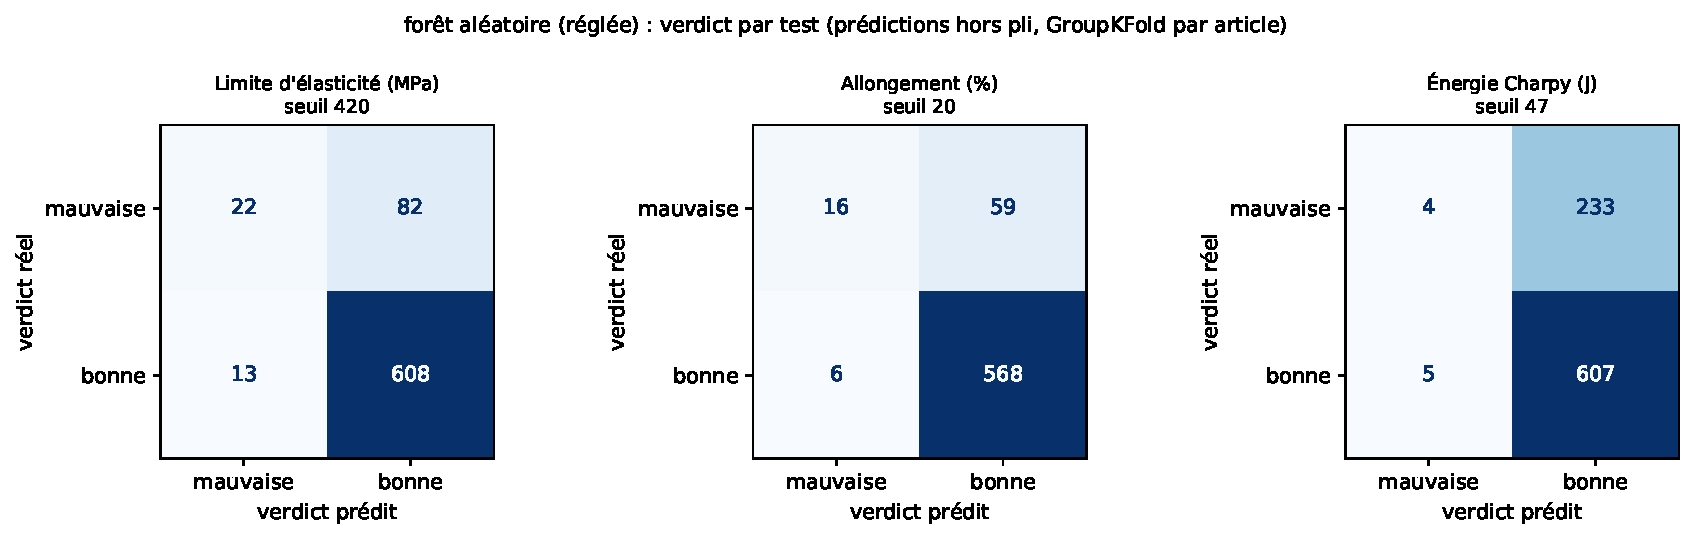
\includegraphics[width=\linewidth]{classification_confusion}
  \caption{Matrices de confusion du verdict, test par test (prédictions hors pli de la
    forêt aléatoire). En haut à droite : les soudures mauvaises acceptées.}
  \label{fig:classif}
\end{figure}

\paragraph{La cause : la régression ramène les extrêmes vers la moyenne.} La forêt
prédit une moyenne de soudures déjà vues ; elle écrase donc les valeurs extrêmes
(section~\ref{sec:modeles}). Elle ne prédit sous le seuil que \SI{5}{\percent} des
lignes en limite d'élasticité, \SI{3}{\percent} en allongement et \SI{1}{\percent} au
Charpy (jamais moins de \SI{31}{\joule}), alors que 14, 12 et \SI{28}{\percent} des
lignes sont réellement sous le seuil. Une soudure faible est prédite « dans la
moyenne », donc au-dessus du seuil. Or la classe « mauvaise » est justement faite de
ces extrêmes bas : un verdict pris sur une valeur prédite hérite de l'écrasement.

\paragraph{En pratique.} En l'état, un verdict « mauvaise » mérite d'être pris au
sérieux ; un verdict « bonne » ne dispense pas d'essais.

\outrouver{notebook \code{modeles.ipynb}, partie 10.3 (tableau par test et figure),
10.4 (verdict global), 10.5 (bilan).}

\subsection{Limites}\label{sec:classif-limites}

\begin{itemize}
  \item \textbf{Une seule norme pour toutes les soudures.} La base contient aussi des
    aciers alliés au chrome et au molybdène, souvent traités thermiquement, qui relèvent
    d'une autre norme (ISO 3580) et d'autres minimums.
  \item \textbf{Un verdict global vérifiable sur peu de soudures.} Seules 182 soudures
    sont mesurées à la fois en traction et au Charpy.
  \item \textbf{Une température Charpy approchée pour l'évaluation.} Le verdict global
    retient l'essai Charpy le plus proche de \SI{-30}{\celsius}, qui en est éloigné de
    \SI{21}{\celsius} en médiane.
\end{itemize}

\afaire{\item Décider avec prudence : ne valider un test que si la prédiction dépasse
    le seuil d'une marge (par exemple une fraction de la RMSE), puis comparer rappel et
    soudures bonnes rejetées.
  \item Comparer à un classifieur direct (forêt de classification sur les étiquettes
    bonne / mauvaise), qui se concentre sur la zone du seuil.
  \item Seuils par famille d'acier (C-Mn et aciers alliés).}

\paragraph{Références.} ISO 2560:2020, \emph{Produits consommables pour le soudage —
Électrodes enrobées pour le soudage manuel à l'arc des aciers non alliés et des aciers à
grains fins — Classification} (système A : symboles de résistance et d'énergie de
rupture, \SI{47}{\joule}). AWS A5.1/A5.1M, \emph{Specification for Carbon Steel
Electrodes for Shielded Metal Arc Welding} (électrode E7018).
